% Created by tikzDevice version 0.12
% !TEX encoding = UTF-8 Unicode
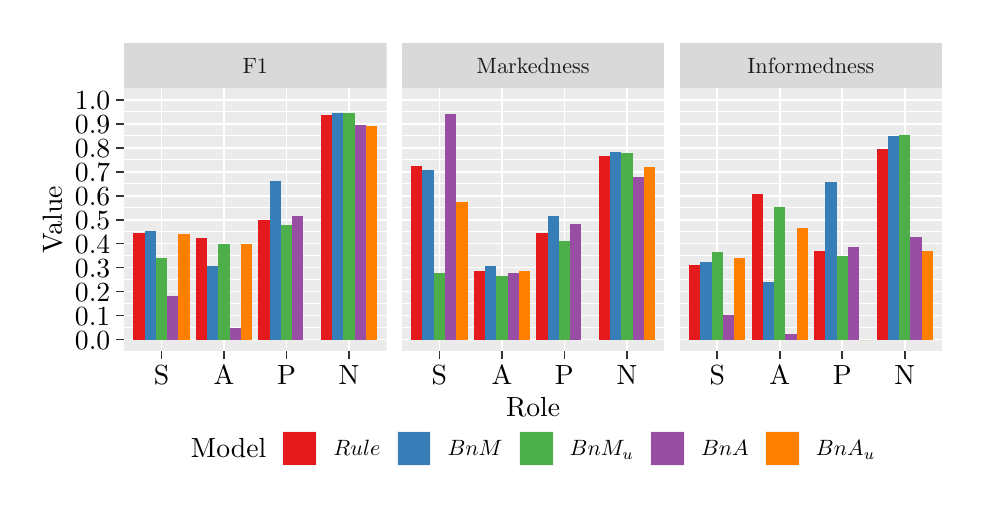
\begin{tikzpicture}[x=1pt,y=1pt]
\definecolor{fillColor}{RGB}{255,255,255}
\path[use as bounding box,fill=fillColor,fill opacity=0.00] (0,0) rectangle (336.00,166.12);
\begin{scope}
\path[clip] (  0.00,  0.00) rectangle (336.00,166.12);
\definecolor{drawColor}{RGB}{255,255,255}
\definecolor{fillColor}{RGB}{255,255,255}

\path[draw=drawColor,line width= 0.6pt,line join=round,line cap=round,fill=fillColor] (  0.00,  0.00) rectangle (336.00,166.12);
\end{scope}
\begin{scope}
\path[clip] ( 34.81, 49.11) rectangle (129.70,144.36);
\definecolor{fillColor}{gray}{0.92}

\path[fill=fillColor] ( 34.81, 49.11) rectangle (129.70,144.36);
\definecolor{drawColor}{RGB}{255,255,255}

\path[draw=drawColor,line width= 0.3pt,line join=round] ( 34.81, 57.77) --
	(129.70, 57.77);

\path[draw=drawColor,line width= 0.3pt,line join=round] ( 34.81, 66.43) --
	(129.70, 66.43);

\path[draw=drawColor,line width= 0.3pt,line join=round] ( 34.81, 75.09) --
	(129.70, 75.09);

\path[draw=drawColor,line width= 0.3pt,line join=round] ( 34.81, 83.75) --
	(129.70, 83.75);

\path[draw=drawColor,line width= 0.3pt,line join=round] ( 34.81, 92.41) --
	(129.70, 92.41);

\path[draw=drawColor,line width= 0.3pt,line join=round] ( 34.81,101.07) --
	(129.70,101.07);

\path[draw=drawColor,line width= 0.3pt,line join=round] ( 34.81,109.73) --
	(129.70,109.73);

\path[draw=drawColor,line width= 0.3pt,line join=round] ( 34.81,118.39) --
	(129.70,118.39);

\path[draw=drawColor,line width= 0.3pt,line join=round] ( 34.81,127.05) --
	(129.70,127.05);

\path[draw=drawColor,line width= 0.3pt,line join=round] ( 34.81,135.71) --
	(129.70,135.71);

\path[draw=drawColor,line width= 0.6pt,line join=round] ( 34.81, 53.44) --
	(129.70, 53.44);

\path[draw=drawColor,line width= 0.6pt,line join=round] ( 34.81, 62.10) --
	(129.70, 62.10);

\path[draw=drawColor,line width= 0.6pt,line join=round] ( 34.81, 70.76) --
	(129.70, 70.76);

\path[draw=drawColor,line width= 0.6pt,line join=round] ( 34.81, 79.42) --
	(129.70, 79.42);

\path[draw=drawColor,line width= 0.6pt,line join=round] ( 34.81, 88.08) --
	(129.70, 88.08);

\path[draw=drawColor,line width= 0.6pt,line join=round] ( 34.81, 96.74) --
	(129.70, 96.74);

\path[draw=drawColor,line width= 0.6pt,line join=round] ( 34.81,105.40) --
	(129.70,105.40);

\path[draw=drawColor,line width= 0.6pt,line join=round] ( 34.81,114.06) --
	(129.70,114.06);

\path[draw=drawColor,line width= 0.6pt,line join=round] ( 34.81,122.72) --
	(129.70,122.72);

\path[draw=drawColor,line width= 0.6pt,line join=round] ( 34.81,131.38) --
	(129.70,131.38);

\path[draw=drawColor,line width= 0.6pt,line join=round] ( 34.81,140.03) --
	(129.70,140.03);

\path[draw=drawColor,line width= 0.6pt,line join=round] ( 48.36, 49.11) --
	( 48.36,144.36);

\path[draw=drawColor,line width= 0.6pt,line join=round] ( 70.96, 49.11) --
	( 70.96,144.36);

\path[draw=drawColor,line width= 0.6pt,line join=round] ( 93.55, 49.11) --
	( 93.55,144.36);

\path[draw=drawColor,line width= 0.6pt,line join=round] (116.15, 49.11) --
	(116.15,144.36);
\definecolor{fillColor}{RGB}{255,127,0}

\path[fill=fillColor] ( 54.46, 53.44) rectangle ( 58.53, 91.52);
\definecolor{fillColor}{RGB}{152,78,163}

\path[fill=fillColor] ( 50.40, 53.44) rectangle ( 54.46, 69.19);
\definecolor{fillColor}{RGB}{77,175,74}

\path[fill=fillColor] ( 46.33, 53.44) rectangle ( 50.40, 83.05);
\definecolor{fillColor}{RGB}{55,126,184}

\path[fill=fillColor] ( 42.26, 53.44) rectangle ( 46.33, 92.77);
\definecolor{fillColor}{RGB}{228,26,28}

\path[fill=fillColor] ( 38.20, 53.44) rectangle ( 42.26, 91.82);
\definecolor{fillColor}{RGB}{255,127,0}

\path[fill=fillColor] ( 77.06, 53.44) rectangle ( 81.13, 87.80);
\definecolor{fillColor}{RGB}{152,78,163}

\path[fill=fillColor] ( 72.99, 53.44) rectangle ( 77.06, 57.62);
\definecolor{fillColor}{RGB}{77,175,74}

\path[fill=fillColor] ( 68.92, 53.44) rectangle ( 72.99, 87.89);
\definecolor{fillColor}{RGB}{55,126,184}

\path[fill=fillColor] ( 64.86, 53.44) rectangle ( 68.92, 79.84);
\definecolor{fillColor}{RGB}{228,26,28}

\path[fill=fillColor] ( 60.79, 53.44) rectangle ( 64.86, 90.29);
\definecolor{fillColor}{RGB}{152,78,163}

\path[fill=fillColor] ( 95.59, 53.44) rectangle ( 99.65, 97.95);
\definecolor{fillColor}{RGB}{77,175,74}

\path[fill=fillColor] ( 91.52, 53.44) rectangle ( 95.59, 94.80);
\definecolor{fillColor}{RGB}{55,126,184}

\path[fill=fillColor] ( 87.45, 53.44) rectangle ( 91.52,110.54);
\definecolor{fillColor}{RGB}{228,26,28}

\path[fill=fillColor] ( 83.38, 53.44) rectangle ( 87.45, 96.53);
\definecolor{fillColor}{RGB}{255,127,0}

\path[fill=fillColor] (122.25, 53.44) rectangle (126.31,130.55);
\definecolor{fillColor}{RGB}{152,78,163}

\path[fill=fillColor] (118.18, 53.44) rectangle (122.25,130.84);
\definecolor{fillColor}{RGB}{77,175,74}

\path[fill=fillColor] (114.11, 53.44) rectangle (118.18,135.17);
\definecolor{fillColor}{RGB}{55,126,184}

\path[fill=fillColor] (110.05, 53.44) rectangle (114.11,135.28);
\definecolor{fillColor}{RGB}{228,26,28}

\path[fill=fillColor] (105.98, 53.44) rectangle (110.05,134.69);
\end{scope}
\begin{scope}
\path[clip] (135.20, 49.11) rectangle (230.10,144.36);
\definecolor{fillColor}{gray}{0.92}

\path[fill=fillColor] (135.20, 49.11) rectangle (230.10,144.36);
\definecolor{drawColor}{RGB}{255,255,255}

\path[draw=drawColor,line width= 0.3pt,line join=round] (135.20, 57.77) --
	(230.10, 57.77);

\path[draw=drawColor,line width= 0.3pt,line join=round] (135.20, 66.43) --
	(230.10, 66.43);

\path[draw=drawColor,line width= 0.3pt,line join=round] (135.20, 75.09) --
	(230.10, 75.09);

\path[draw=drawColor,line width= 0.3pt,line join=round] (135.20, 83.75) --
	(230.10, 83.75);

\path[draw=drawColor,line width= 0.3pt,line join=round] (135.20, 92.41) --
	(230.10, 92.41);

\path[draw=drawColor,line width= 0.3pt,line join=round] (135.20,101.07) --
	(230.10,101.07);

\path[draw=drawColor,line width= 0.3pt,line join=round] (135.20,109.73) --
	(230.10,109.73);

\path[draw=drawColor,line width= 0.3pt,line join=round] (135.20,118.39) --
	(230.10,118.39);

\path[draw=drawColor,line width= 0.3pt,line join=round] (135.20,127.05) --
	(230.10,127.05);

\path[draw=drawColor,line width= 0.3pt,line join=round] (135.20,135.71) --
	(230.10,135.71);

\path[draw=drawColor,line width= 0.6pt,line join=round] (135.20, 53.44) --
	(230.10, 53.44);

\path[draw=drawColor,line width= 0.6pt,line join=round] (135.20, 62.10) --
	(230.10, 62.10);

\path[draw=drawColor,line width= 0.6pt,line join=round] (135.20, 70.76) --
	(230.10, 70.76);

\path[draw=drawColor,line width= 0.6pt,line join=round] (135.20, 79.42) --
	(230.10, 79.42);

\path[draw=drawColor,line width= 0.6pt,line join=round] (135.20, 88.08) --
	(230.10, 88.08);

\path[draw=drawColor,line width= 0.6pt,line join=round] (135.20, 96.74) --
	(230.10, 96.74);

\path[draw=drawColor,line width= 0.6pt,line join=round] (135.20,105.40) --
	(230.10,105.40);

\path[draw=drawColor,line width= 0.6pt,line join=round] (135.20,114.06) --
	(230.10,114.06);

\path[draw=drawColor,line width= 0.6pt,line join=round] (135.20,122.72) --
	(230.10,122.72);

\path[draw=drawColor,line width= 0.6pt,line join=round] (135.20,131.38) --
	(230.10,131.38);

\path[draw=drawColor,line width= 0.6pt,line join=round] (135.20,140.03) --
	(230.10,140.03);

\path[draw=drawColor,line width= 0.6pt,line join=round] (148.76, 49.11) --
	(148.76,144.36);

\path[draw=drawColor,line width= 0.6pt,line join=round] (171.36, 49.11) --
	(171.36,144.36);

\path[draw=drawColor,line width= 0.6pt,line join=round] (193.95, 49.11) --
	(193.95,144.36);

\path[draw=drawColor,line width= 0.6pt,line join=round] (216.55, 49.11) --
	(216.55,144.36);
\definecolor{fillColor}{RGB}{255,127,0}

\path[fill=fillColor] (154.86, 53.44) rectangle (158.93,103.08);
\definecolor{fillColor}{RGB}{152,78,163}

\path[fill=fillColor] (150.79, 53.44) rectangle (154.86,134.95);
\definecolor{fillColor}{RGB}{77,175,74}

\path[fill=fillColor] (146.73, 53.44) rectangle (150.79, 77.55);
\definecolor{fillColor}{RGB}{55,126,184}

\path[fill=fillColor] (142.66, 53.44) rectangle (146.73,114.73);
\definecolor{fillColor}{RGB}{228,26,28}

\path[fill=fillColor] (138.59, 53.44) rectangle (142.66,116.05);
\definecolor{fillColor}{RGB}{255,127,0}

\path[fill=fillColor] (177.46, 53.44) rectangle (181.52, 78.25);
\definecolor{fillColor}{RGB}{152,78,163}

\path[fill=fillColor] (173.39, 53.44) rectangle (177.46, 77.57);
\definecolor{fillColor}{RGB}{77,175,74}

\path[fill=fillColor] (169.32, 53.44) rectangle (173.39, 76.37);
\definecolor{fillColor}{RGB}{55,126,184}

\path[fill=fillColor] (165.25, 53.44) rectangle (169.32, 80.08);
\definecolor{fillColor}{RGB}{228,26,28}

\path[fill=fillColor] (161.19, 53.44) rectangle (165.25, 78.21);
\definecolor{fillColor}{RGB}{152,78,163}

\path[fill=fillColor] (195.98, 53.44) rectangle (200.05, 95.04);
\definecolor{fillColor}{RGB}{77,175,74}

\path[fill=fillColor] (191.92, 53.44) rectangle (195.98, 89.04);
\definecolor{fillColor}{RGB}{55,126,184}

\path[fill=fillColor] (187.85, 53.44) rectangle (191.92, 98.00);
\definecolor{fillColor}{RGB}{228,26,28}

\path[fill=fillColor] (183.78, 53.44) rectangle (187.85, 91.97);
\definecolor{fillColor}{RGB}{255,127,0}

\path[fill=fillColor] (222.65, 53.44) rectangle (226.71,115.68);
\definecolor{fillColor}{RGB}{152,78,163}

\path[fill=fillColor] (218.58, 53.44) rectangle (222.65,112.27);
\definecolor{fillColor}{RGB}{77,175,74}

\path[fill=fillColor] (214.51, 53.44) rectangle (218.58,120.72);
\definecolor{fillColor}{RGB}{55,126,184}

\path[fill=fillColor] (210.44, 53.44) rectangle (214.51,121.16);
\definecolor{fillColor}{RGB}{228,26,28}

\path[fill=fillColor] (206.38, 53.44) rectangle (210.44,119.66);
\end{scope}
\begin{scope}
\path[clip] (235.60, 49.11) rectangle (330.50,144.36);
\definecolor{fillColor}{gray}{0.92}

\path[fill=fillColor] (235.60, 49.11) rectangle (330.50,144.36);
\definecolor{drawColor}{RGB}{255,255,255}

\path[draw=drawColor,line width= 0.3pt,line join=round] (235.60, 57.77) --
	(330.50, 57.77);

\path[draw=drawColor,line width= 0.3pt,line join=round] (235.60, 66.43) --
	(330.50, 66.43);

\path[draw=drawColor,line width= 0.3pt,line join=round] (235.60, 75.09) --
	(330.50, 75.09);

\path[draw=drawColor,line width= 0.3pt,line join=round] (235.60, 83.75) --
	(330.50, 83.75);

\path[draw=drawColor,line width= 0.3pt,line join=round] (235.60, 92.41) --
	(330.50, 92.41);

\path[draw=drawColor,line width= 0.3pt,line join=round] (235.60,101.07) --
	(330.50,101.07);

\path[draw=drawColor,line width= 0.3pt,line join=round] (235.60,109.73) --
	(330.50,109.73);

\path[draw=drawColor,line width= 0.3pt,line join=round] (235.60,118.39) --
	(330.50,118.39);

\path[draw=drawColor,line width= 0.3pt,line join=round] (235.60,127.05) --
	(330.50,127.05);

\path[draw=drawColor,line width= 0.3pt,line join=round] (235.60,135.71) --
	(330.50,135.71);

\path[draw=drawColor,line width= 0.6pt,line join=round] (235.60, 53.44) --
	(330.50, 53.44);

\path[draw=drawColor,line width= 0.6pt,line join=round] (235.60, 62.10) --
	(330.50, 62.10);

\path[draw=drawColor,line width= 0.6pt,line join=round] (235.60, 70.76) --
	(330.50, 70.76);

\path[draw=drawColor,line width= 0.6pt,line join=round] (235.60, 79.42) --
	(330.50, 79.42);

\path[draw=drawColor,line width= 0.6pt,line join=round] (235.60, 88.08) --
	(330.50, 88.08);

\path[draw=drawColor,line width= 0.6pt,line join=round] (235.60, 96.74) --
	(330.50, 96.74);

\path[draw=drawColor,line width= 0.6pt,line join=round] (235.60,105.40) --
	(330.50,105.40);

\path[draw=drawColor,line width= 0.6pt,line join=round] (235.60,114.06) --
	(330.50,114.06);

\path[draw=drawColor,line width= 0.6pt,line join=round] (235.60,122.72) --
	(330.50,122.72);

\path[draw=drawColor,line width= 0.6pt,line join=round] (235.60,131.38) --
	(330.50,131.38);

\path[draw=drawColor,line width= 0.6pt,line join=round] (235.60,140.03) --
	(330.50,140.03);

\path[draw=drawColor,line width= 0.6pt,line join=round] (249.16, 49.11) --
	(249.16,144.36);

\path[draw=drawColor,line width= 0.6pt,line join=round] (271.75, 49.11) --
	(271.75,144.36);

\path[draw=drawColor,line width= 0.6pt,line join=round] (294.35, 49.11) --
	(294.35,144.36);

\path[draw=drawColor,line width= 0.6pt,line join=round] (316.94, 49.11) --
	(316.94,144.36);
\definecolor{fillColor}{RGB}{255,127,0}

\path[fill=fillColor] (255.26, 53.44) rectangle (259.33, 82.92);
\definecolor{fillColor}{RGB}{152,78,163}

\path[fill=fillColor] (251.19, 53.44) rectangle (255.26, 62.12);
\definecolor{fillColor}{RGB}{77,175,74}

\path[fill=fillColor] (247.13, 53.44) rectangle (251.19, 85.15);
\definecolor{fillColor}{RGB}{55,126,184}

\path[fill=fillColor] (243.06, 53.44) rectangle (247.13, 81.61);
\definecolor{fillColor}{RGB}{228,26,28}

\path[fill=fillColor] (238.99, 53.44) rectangle (243.06, 80.41);
\definecolor{fillColor}{RGB}{255,127,0}

\path[fill=fillColor] (277.85, 53.44) rectangle (281.92, 93.83);
\definecolor{fillColor}{RGB}{152,78,163}

\path[fill=fillColor] (273.79, 53.44) rectangle (277.85, 55.43);
\definecolor{fillColor}{RGB}{77,175,74}

\path[fill=fillColor] (269.72, 53.44) rectangle (273.79,101.17);
\definecolor{fillColor}{RGB}{55,126,184}

\path[fill=fillColor] (265.65, 53.44) rectangle (269.72, 74.24);
\definecolor{fillColor}{RGB}{228,26,28}

\path[fill=fillColor] (261.59, 53.44) rectangle (265.65,106.08);
\definecolor{fillColor}{RGB}{255,127,0}

\path[fill=fillColor] (300.45, 53.44) rectangle (304.52, 53.44);
\definecolor{fillColor}{RGB}{152,78,163}

\path[fill=fillColor] (296.38, 53.44) rectangle (300.45, 86.74);
\definecolor{fillColor}{RGB}{77,175,74}

\path[fill=fillColor] (292.31, 53.44) rectangle (296.38, 83.71);
\definecolor{fillColor}{RGB}{55,126,184}

\path[fill=fillColor] (288.25, 53.44) rectangle (292.31,110.37);
\definecolor{fillColor}{RGB}{228,26,28}

\path[fill=fillColor] (284.18, 53.44) rectangle (288.25, 85.46);
\definecolor{fillColor}{RGB}{255,127,0}

\path[fill=fillColor] (323.04, 53.44) rectangle (327.11, 85.50);
\definecolor{fillColor}{RGB}{152,78,163}

\path[fill=fillColor] (318.98, 53.44) rectangle (323.04, 90.46);
\definecolor{fillColor}{RGB}{77,175,74}

\path[fill=fillColor] (314.91, 53.44) rectangle (318.98,127.47);
\definecolor{fillColor}{RGB}{55,126,184}

\path[fill=fillColor] (310.84, 53.44) rectangle (314.91,127.08);
\definecolor{fillColor}{RGB}{228,26,28}

\path[fill=fillColor] (306.78, 53.44) rectangle (310.84,122.13);
\end{scope}
\begin{scope}
\path[clip] ( 34.81,144.36) rectangle (129.70,160.62);
\definecolor{fillColor}{gray}{0.85}

\path[fill=fillColor] ( 34.81,144.36) rectangle (129.70,160.62);
\definecolor{drawColor}{gray}{0.10}

\node[text=drawColor,anchor=base,inner sep=0pt, outer sep=0pt, scale=  0.80] at ( 82.25,149.74) {F1};
\end{scope}
\begin{scope}
\path[clip] (135.20,144.36) rectangle (230.10,160.62);
\definecolor{fillColor}{gray}{0.85}

\path[fill=fillColor] (135.20,144.36) rectangle (230.10,160.62);
\definecolor{drawColor}{gray}{0.10}

\node[text=drawColor,anchor=base,inner sep=0pt, outer sep=0pt, scale=  0.80] at (182.65,149.74) {Markedness};
\end{scope}
\begin{scope}
\path[clip] (235.60,144.36) rectangle (330.50,160.62);
\definecolor{fillColor}{gray}{0.85}

\path[fill=fillColor] (235.60,144.36) rectangle (330.50,160.62);
\definecolor{drawColor}{gray}{0.10}

\node[text=drawColor,anchor=base,inner sep=0pt, outer sep=0pt, scale=  0.80] at (283.05,149.74) {Informedness};
\end{scope}
\begin{scope}
\path[clip] (  0.00,  0.00) rectangle (336.00,166.12);
\definecolor{drawColor}{gray}{0.20}

\path[draw=drawColor,line width= 0.6pt,line join=round] ( 48.36, 46.36) --
	( 48.36, 49.11);

\path[draw=drawColor,line width= 0.6pt,line join=round] ( 70.96, 46.36) --
	( 70.96, 49.11);

\path[draw=drawColor,line width= 0.6pt,line join=round] ( 93.55, 46.36) --
	( 93.55, 49.11);

\path[draw=drawColor,line width= 0.6pt,line join=round] (116.15, 46.36) --
	(116.15, 49.11);
\end{scope}
\begin{scope}
\path[clip] (  0.00,  0.00) rectangle (336.00,166.12);
\definecolor{drawColor}{RGB}{0,0,0}

\node[text=drawColor,anchor=base,inner sep=0pt, outer sep=0pt, scale=  1.00] at ( 48.36, 37.27) {S};

\node[text=drawColor,anchor=base,inner sep=0pt, outer sep=0pt, scale=  1.00] at ( 70.96, 37.27) {A};

\node[text=drawColor,anchor=base,inner sep=0pt, outer sep=0pt, scale=  1.00] at ( 93.55, 37.27) {P};

\node[text=drawColor,anchor=base,inner sep=0pt, outer sep=0pt, scale=  1.00] at (116.15, 37.27) {N};
\end{scope}
\begin{scope}
\path[clip] (  0.00,  0.00) rectangle (336.00,166.12);
\definecolor{drawColor}{gray}{0.20}

\path[draw=drawColor,line width= 0.6pt,line join=round] (148.76, 46.36) --
	(148.76, 49.11);

\path[draw=drawColor,line width= 0.6pt,line join=round] (171.36, 46.36) --
	(171.36, 49.11);

\path[draw=drawColor,line width= 0.6pt,line join=round] (193.95, 46.36) --
	(193.95, 49.11);

\path[draw=drawColor,line width= 0.6pt,line join=round] (216.55, 46.36) --
	(216.55, 49.11);
\end{scope}
\begin{scope}
\path[clip] (  0.00,  0.00) rectangle (336.00,166.12);
\definecolor{drawColor}{RGB}{0,0,0}

\node[text=drawColor,anchor=base,inner sep=0pt, outer sep=0pt, scale=  1.00] at (148.76, 37.27) {S};

\node[text=drawColor,anchor=base,inner sep=0pt, outer sep=0pt, scale=  1.00] at (171.36, 37.27) {A};

\node[text=drawColor,anchor=base,inner sep=0pt, outer sep=0pt, scale=  1.00] at (193.95, 37.27) {P};

\node[text=drawColor,anchor=base,inner sep=0pt, outer sep=0pt, scale=  1.00] at (216.55, 37.27) {N};
\end{scope}
\begin{scope}
\path[clip] (  0.00,  0.00) rectangle (336.00,166.12);
\definecolor{drawColor}{gray}{0.20}

\path[draw=drawColor,line width= 0.6pt,line join=round] (249.16, 46.36) --
	(249.16, 49.11);

\path[draw=drawColor,line width= 0.6pt,line join=round] (271.75, 46.36) --
	(271.75, 49.11);

\path[draw=drawColor,line width= 0.6pt,line join=round] (294.35, 46.36) --
	(294.35, 49.11);

\path[draw=drawColor,line width= 0.6pt,line join=round] (316.94, 46.36) --
	(316.94, 49.11);
\end{scope}
\begin{scope}
\path[clip] (  0.00,  0.00) rectangle (336.00,166.12);
\definecolor{drawColor}{RGB}{0,0,0}

\node[text=drawColor,anchor=base,inner sep=0pt, outer sep=0pt, scale=  1.00] at (249.16, 37.27) {S};

\node[text=drawColor,anchor=base,inner sep=0pt, outer sep=0pt, scale=  1.00] at (271.75, 37.27) {A};

\node[text=drawColor,anchor=base,inner sep=0pt, outer sep=0pt, scale=  1.00] at (294.35, 37.27) {P};

\node[text=drawColor,anchor=base,inner sep=0pt, outer sep=0pt, scale=  1.00] at (316.94, 37.27) {N};
\end{scope}
\begin{scope}
\path[clip] (  0.00,  0.00) rectangle (336.00,166.12);
\definecolor{drawColor}{RGB}{0,0,0}

\node[text=drawColor,anchor=base east,inner sep=0pt, outer sep=0pt, scale=  1.00] at ( 29.86, 50.00) {0.0};

\node[text=drawColor,anchor=base east,inner sep=0pt, outer sep=0pt, scale=  1.00] at ( 29.86, 58.66) {0.1};

\node[text=drawColor,anchor=base east,inner sep=0pt, outer sep=0pt, scale=  1.00] at ( 29.86, 67.32) {0.2};

\node[text=drawColor,anchor=base east,inner sep=0pt, outer sep=0pt, scale=  1.00] at ( 29.86, 75.98) {0.3};

\node[text=drawColor,anchor=base east,inner sep=0pt, outer sep=0pt, scale=  1.00] at ( 29.86, 84.64) {0.4};

\node[text=drawColor,anchor=base east,inner sep=0pt, outer sep=0pt, scale=  1.00] at ( 29.86, 93.29) {0.5};

\node[text=drawColor,anchor=base east,inner sep=0pt, outer sep=0pt, scale=  1.00] at ( 29.86,101.95) {0.6};

\node[text=drawColor,anchor=base east,inner sep=0pt, outer sep=0pt, scale=  1.00] at ( 29.86,110.61) {0.7};

\node[text=drawColor,anchor=base east,inner sep=0pt, outer sep=0pt, scale=  1.00] at ( 29.86,119.27) {0.8};

\node[text=drawColor,anchor=base east,inner sep=0pt, outer sep=0pt, scale=  1.00] at ( 29.86,127.93) {0.9};

\node[text=drawColor,anchor=base east,inner sep=0pt, outer sep=0pt, scale=  1.00] at ( 29.86,136.59) {1.0};
\end{scope}
\begin{scope}
\path[clip] (  0.00,  0.00) rectangle (336.00,166.12);
\definecolor{drawColor}{gray}{0.20}

\path[draw=drawColor,line width= 0.6pt,line join=round] ( 32.06, 53.44) --
	( 34.81, 53.44);

\path[draw=drawColor,line width= 0.6pt,line join=round] ( 32.06, 62.10) --
	( 34.81, 62.10);

\path[draw=drawColor,line width= 0.6pt,line join=round] ( 32.06, 70.76) --
	( 34.81, 70.76);

\path[draw=drawColor,line width= 0.6pt,line join=round] ( 32.06, 79.42) --
	( 34.81, 79.42);

\path[draw=drawColor,line width= 0.6pt,line join=round] ( 32.06, 88.08) --
	( 34.81, 88.08);

\path[draw=drawColor,line width= 0.6pt,line join=round] ( 32.06, 96.74) --
	( 34.81, 96.74);

\path[draw=drawColor,line width= 0.6pt,line join=round] ( 32.06,105.40) --
	( 34.81,105.40);

\path[draw=drawColor,line width= 0.6pt,line join=round] ( 32.06,114.06) --
	( 34.81,114.06);

\path[draw=drawColor,line width= 0.6pt,line join=round] ( 32.06,122.72) --
	( 34.81,122.72);

\path[draw=drawColor,line width= 0.6pt,line join=round] ( 32.06,131.38) --
	( 34.81,131.38);

\path[draw=drawColor,line width= 0.6pt,line join=round] ( 32.06,140.03) --
	( 34.81,140.03);
\end{scope}
\begin{scope}
\path[clip] (  0.00,  0.00) rectangle (336.00,166.12);
\definecolor{drawColor}{RGB}{0,0,0}

\node[text=drawColor,anchor=base,inner sep=0pt, outer sep=0pt, scale=  1.00] at (182.65, 25.69) {Role};
\end{scope}
\begin{scope}
\path[clip] (  0.00,  0.00) rectangle (336.00,166.12);
\definecolor{drawColor}{RGB}{0,0,0}

\node[text=drawColor,rotate= 90.00,anchor=base,inner sep=0pt, outer sep=0pt, scale=  1.00] at ( 12.39, 96.74) {Value};
\end{scope}
\begin{scope}
\path[clip] (  0.00,  0.00) rectangle (336.00,166.12);
\definecolor{fillColor}{RGB}{255,255,255}

\path[fill=fillColor] ( 57.01,  5.50) rectangle (308.30, 22.75);
\end{scope}
\begin{scope}
\path[clip] (  0.00,  0.00) rectangle (336.00,166.12);
\definecolor{drawColor}{RGB}{0,0,0}

\node[text=drawColor,anchor=base west,inner sep=0pt, outer sep=0pt, scale=  1.00] at ( 59.01, 10.68) {Model};
\end{scope}
\begin{scope}
\path[clip] (  0.00,  0.00) rectangle (336.00,166.12);
\definecolor{drawColor}{RGB}{255,255,255}
\definecolor{fillColor}{gray}{0.95}

\path[draw=drawColor,line width= 0.6pt,line join=round,line cap=round,fill=fillColor] ( 91.72,  7.50) rectangle (104.97, 20.75);
\end{scope}
\begin{scope}
\path[clip] (  0.00,  0.00) rectangle (336.00,166.12);
\definecolor{fillColor}{RGB}{228,26,28}

\path[fill=fillColor] ( 92.43,  8.21) rectangle (104.26, 20.04);
\end{scope}
\begin{scope}
\path[clip] (  0.00,  0.00) rectangle (336.00,166.12);
\definecolor{drawColor}{RGB}{255,255,255}
\definecolor{fillColor}{gray}{0.95}

\path[draw=drawColor,line width= 0.6pt,line join=round,line cap=round,fill=fillColor] (132.96,  7.50) rectangle (146.21, 20.75);
\end{scope}
\begin{scope}
\path[clip] (  0.00,  0.00) rectangle (336.00,166.12);
\definecolor{fillColor}{RGB}{55,126,184}

\path[fill=fillColor] (133.67,  8.21) rectangle (145.49, 20.04);
\end{scope}
\begin{scope}
\path[clip] (  0.00,  0.00) rectangle (336.00,166.12);
\definecolor{drawColor}{RGB}{255,255,255}
\definecolor{fillColor}{gray}{0.95}

\path[draw=drawColor,line width= 0.6pt,line join=round,line cap=round,fill=fillColor] (177.11,  7.50) rectangle (190.36, 20.75);
\end{scope}
\begin{scope}
\path[clip] (  0.00,  0.00) rectangle (336.00,166.12);
\definecolor{fillColor}{RGB}{77,175,74}

\path[fill=fillColor] (177.82,  8.21) rectangle (189.65, 20.04);
\end{scope}
\begin{scope}
\path[clip] (  0.00,  0.00) rectangle (336.00,166.12);
\definecolor{drawColor}{RGB}{255,255,255}
\definecolor{fillColor}{gray}{0.95}

\path[draw=drawColor,line width= 0.6pt,line join=round,line cap=round,fill=fillColor] (224.58,  7.50) rectangle (237.82, 20.75);
\end{scope}
\begin{scope}
\path[clip] (  0.00,  0.00) rectangle (336.00,166.12);
\definecolor{fillColor}{RGB}{152,78,163}

\path[fill=fillColor] (225.29,  8.21) rectangle (237.11, 20.04);
\end{scope}
\begin{scope}
\path[clip] (  0.00,  0.00) rectangle (336.00,166.12);
\definecolor{drawColor}{RGB}{255,255,255}
\definecolor{fillColor}{gray}{0.95}

\path[draw=drawColor,line width= 0.6pt,line join=round,line cap=round,fill=fillColor] (266.10,  7.50) rectangle (279.35, 20.75);
\end{scope}
\begin{scope}
\path[clip] (  0.00,  0.00) rectangle (336.00,166.12);
\definecolor{fillColor}{RGB}{255,127,0}

\path[fill=fillColor] (266.81,  8.21) rectangle (278.63, 20.04);
\end{scope}
\begin{scope}
\path[clip] (  0.00,  0.00) rectangle (336.00,166.12);
\definecolor{drawColor}{RGB}{0,0,0}

\node[text=drawColor,anchor=base west,inner sep=0pt, outer sep=0pt, scale=  0.80] at (110.47, 11.37) {\(Rule\)};
\end{scope}
\begin{scope}
\path[clip] (  0.00,  0.00) rectangle (336.00,166.12);
\definecolor{drawColor}{RGB}{0,0,0}

\node[text=drawColor,anchor=base west,inner sep=0pt, outer sep=0pt, scale=  0.80] at (151.71, 11.37) {\(BnM\)};
\end{scope}
\begin{scope}
\path[clip] (  0.00,  0.00) rectangle (336.00,166.12);
\definecolor{drawColor}{RGB}{0,0,0}

\node[text=drawColor,anchor=base west,inner sep=0pt, outer sep=0pt, scale=  0.80] at (195.86, 11.37) {\(BnM_u\)};
\end{scope}
\begin{scope}
\path[clip] (  0.00,  0.00) rectangle (336.00,166.12);
\definecolor{drawColor}{RGB}{0,0,0}

\node[text=drawColor,anchor=base west,inner sep=0pt, outer sep=0pt, scale=  0.80] at (243.32, 11.37) {\(BnA\)};
\end{scope}
\begin{scope}
\path[clip] (  0.00,  0.00) rectangle (336.00,166.12);
\definecolor{drawColor}{RGB}{0,0,0}

\node[text=drawColor,anchor=base west,inner sep=0pt, outer sep=0pt, scale=  0.80] at (284.85, 11.37) {\(BnA_u\)};
\end{scope}
\end{tikzpicture}
